
\documentclass[a4paper,landscape,11pt]{article}

\usepackage[margin=1.0cm]{geometry}
\usepackage{tikz}
\usetikzlibrary{shapes.geometric}

\pagestyle{empty}

\begin{document}
	
	\begin{center}
		{\Huge\bfseries StudyFlow}\\[3pt]
		{\Large Entity Relationship Diagram}\\[3pt]
		{\normalsize Core data model for the StudyFlow productivity application}
	\end{center}
	
	\vspace{0.2cm}
	
	\begin{center}
		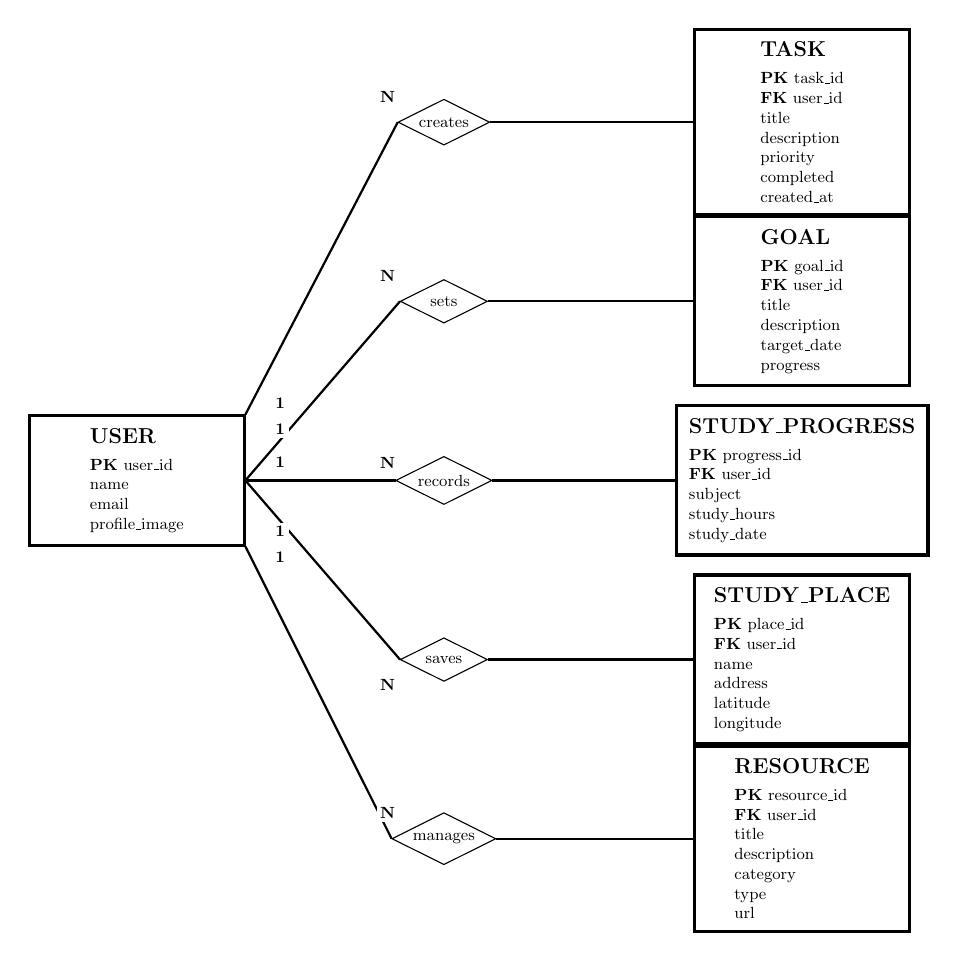
\begin{tikzpicture}[scale=0.65,transform shape]
			
			\tikzset{
				entity/.style={
					draw,
					rectangle,
					very thick,
					minimum width=4.2cm,
					align=left,
					inner sep=7pt,
					font=\small
				},
				relation/.style={
					draw,
					diamond,
					aspect=2,
					minimum width=1.7cm,
					minimum height=0.85cm,
					inner sep=2pt,
					font=\small
				},
				cardinality/.style={
					fill=white,
					inner sep=2pt,
					font=\bfseries\small
				}
			}
			
			% USER
			\node[entity] (user) at (-8,0) {
				\textbf{\large USER}\\[4pt]
				\textbf{PK} user\_id\\
				name\\
				email\\
				profile\_image
			};
			
			% TASK
			\node[entity] (task) at (5,7) {
				\textbf{\large TASK}\\[4pt]
				\textbf{PK} task\_id\\
				\textbf{FK} user\_id\\
				title\\
				description\\
				priority\\
				completed\\
				created\_at
			};
			
			% GOAL
			\node[entity] (goal) at (5,3.5) {
				\textbf{\large GOAL}\\[4pt]
				\textbf{PK} goal\_id\\
				\textbf{FK} user\_id\\
				title\\
				description\\
				target\_date\\
				progress
			};
			
			% STUDY PROGRESS
			\node[entity] (progress) at (5,0) {
				\textbf{\large STUDY\_PROGRESS}\\[4pt]
				\textbf{PK} progress\_id\\
				\textbf{FK} user\_id\\
				subject\\
				study\_hours\\
				study\_date
			};
			
			% STUDY PLACE
			\node[entity] (place) at (5,-3.5) {
				\textbf{\large STUDY\_PLACE}\\[4pt]
				\textbf{PK} place\_id\\
				\textbf{FK} user\_id\\
				name\\
				address\\
				latitude\\
				longitude
			};
			
			% RESOURCE
			\node[entity] (resource) at (5,-7) {
				\textbf{\large RESOURCE}\\[4pt]
				\textbf{PK} resource\_id\\
				\textbf{FK} user\_id\\
				title\\
				description\\
				category\\
				type\\
				url
			};
			
			% RELATIONSHIP DIAMONDS
			\node[relation] (creates) at (-2,7) {creates};
			\node[relation] (sets) at (-2,3.5) {sets};
			\node[relation] (records) at (-2,0) {records};
			\node[relation] (saves) at (-2,-3.5) {saves};
			\node[relation] (manages) at (-2,-7) {manages};
			
			% USER TO RELATIONSHIPS
			\draw[thick] (user.north east) -- (creates.west);
			\draw[thick] (user.east) -- (sets.west);
			\draw[thick] (user.east) -- (records.west);
			\draw[thick] (user.east) -- (saves.west);
			\draw[thick] (user.south east) -- (manages.west);
			
			% RELATIONSHIPS TO ENTITIES
			\draw[thick] (creates.east) -- (task.west);
			\draw[thick] (sets.east) -- (goal.west);
			\draw[thick] (records.east) -- (progress.west);
			\draw[thick] (saves.east) -- (place.west);
			\draw[thick] (manages.east) -- (resource.west);
			
			% CARDINALITIES
			\node[cardinality] at (-5.2,1.5) {1};
			\node[cardinality] at (-3.1,7.5) {N};
			
			\node[cardinality] at (-5.2,1.0) {1};
			\node[cardinality] at (-3.1,4.0) {N};
			
			\node[cardinality] at (-5.2,0.35) {1};
			\node[cardinality] at (-3.1,0.35) {N};
			
			\node[cardinality] at (-5.2,-1.0) {1};
			\node[cardinality] at (-3.1,-4.0) {N};
			
			\node[cardinality] at (-5.2,-1.5) {1};
			\node[cardinality] at (-3.1,-6.5) {N};
			
		\end{tikzpicture}
	\end{center}
	
	\vspace{0.1cm}
	
	\begin{center}
		\fbox{
			\parbox{0.8\textwidth}{
				\centering
				\textbf{Legend:}
				PK = Primary Key
				\qquad
				FK = Foreign Key
				\qquad
				1:N = One-to-Many Relationship
			}
		}
		
		\vspace{0.15cm}
		{\small\itshape StudyFlow --- CSE 510 Mobile Application Development Lab}
	\end{center}
	
\end{document}